% Options for packages loaded elsewhere
\PassOptionsToPackage{unicode}{hyperref}
\PassOptionsToPackage{hyphens}{url}
%
\documentclass[
]{book}
\usepackage{lmodern}
\usepackage{amssymb,amsmath}
\usepackage{ifxetex,ifluatex}
\ifnum 0\ifxetex 1\fi\ifluatex 1\fi=0 % if pdftex
  \usepackage[T1]{fontenc}
  \usepackage[utf8]{inputenc}
  \usepackage{textcomp} % provide euro and other symbols
\else % if luatex or xetex
  \usepackage{unicode-math}
  \defaultfontfeatures{Scale=MatchLowercase}
  \defaultfontfeatures[\rmfamily]{Ligatures=TeX,Scale=1}
\fi
% Use upquote if available, for straight quotes in verbatim environments
\IfFileExists{upquote.sty}{\usepackage{upquote}}{}
\IfFileExists{microtype.sty}{% use microtype if available
  \usepackage[]{microtype}
  \UseMicrotypeSet[protrusion]{basicmath} % disable protrusion for tt fonts
}{}
\makeatletter
\@ifundefined{KOMAClassName}{% if non-KOMA class
  \IfFileExists{parskip.sty}{%
    \usepackage{parskip}
  }{% else
    \setlength{\parindent}{0pt}
    \setlength{\parskip}{6pt plus 2pt minus 1pt}}
}{% if KOMA class
  \KOMAoptions{parskip=half}}
\makeatother
\usepackage{xcolor}
\IfFileExists{xurl.sty}{\usepackage{xurl}}{} % add URL line breaks if available
\IfFileExists{bookmark.sty}{\usepackage{bookmark}}{\usepackage{hyperref}}
\hypersetup{
  pdftitle={Apuntes de Economía y Administración de Empresas},
  pdfauthor={Saúl Torres-Ortega},
  hidelinks,
  pdfcreator={LaTeX via pandoc}}
\urlstyle{same} % disable monospaced font for URLs
\usepackage{color}
\usepackage{fancyvrb}
\newcommand{\VerbBar}{|}
\newcommand{\VERB}{\Verb[commandchars=\\\{\}]}
\DefineVerbatimEnvironment{Highlighting}{Verbatim}{commandchars=\\\{\}}
% Add ',fontsize=\small' for more characters per line
\usepackage{framed}
\definecolor{shadecolor}{RGB}{248,248,248}
\newenvironment{Shaded}{\begin{snugshade}}{\end{snugshade}}
\newcommand{\AlertTok}[1]{\textcolor[rgb]{0.94,0.16,0.16}{#1}}
\newcommand{\AnnotationTok}[1]{\textcolor[rgb]{0.56,0.35,0.01}{\textbf{\textit{#1}}}}
\newcommand{\AttributeTok}[1]{\textcolor[rgb]{0.77,0.63,0.00}{#1}}
\newcommand{\BaseNTok}[1]{\textcolor[rgb]{0.00,0.00,0.81}{#1}}
\newcommand{\BuiltInTok}[1]{#1}
\newcommand{\CharTok}[1]{\textcolor[rgb]{0.31,0.60,0.02}{#1}}
\newcommand{\CommentTok}[1]{\textcolor[rgb]{0.56,0.35,0.01}{\textit{#1}}}
\newcommand{\CommentVarTok}[1]{\textcolor[rgb]{0.56,0.35,0.01}{\textbf{\textit{#1}}}}
\newcommand{\ConstantTok}[1]{\textcolor[rgb]{0.00,0.00,0.00}{#1}}
\newcommand{\ControlFlowTok}[1]{\textcolor[rgb]{0.13,0.29,0.53}{\textbf{#1}}}
\newcommand{\DataTypeTok}[1]{\textcolor[rgb]{0.13,0.29,0.53}{#1}}
\newcommand{\DecValTok}[1]{\textcolor[rgb]{0.00,0.00,0.81}{#1}}
\newcommand{\DocumentationTok}[1]{\textcolor[rgb]{0.56,0.35,0.01}{\textbf{\textit{#1}}}}
\newcommand{\ErrorTok}[1]{\textcolor[rgb]{0.64,0.00,0.00}{\textbf{#1}}}
\newcommand{\ExtensionTok}[1]{#1}
\newcommand{\FloatTok}[1]{\textcolor[rgb]{0.00,0.00,0.81}{#1}}
\newcommand{\FunctionTok}[1]{\textcolor[rgb]{0.00,0.00,0.00}{#1}}
\newcommand{\ImportTok}[1]{#1}
\newcommand{\InformationTok}[1]{\textcolor[rgb]{0.56,0.35,0.01}{\textbf{\textit{#1}}}}
\newcommand{\KeywordTok}[1]{\textcolor[rgb]{0.13,0.29,0.53}{\textbf{#1}}}
\newcommand{\NormalTok}[1]{#1}
\newcommand{\OperatorTok}[1]{\textcolor[rgb]{0.81,0.36,0.00}{\textbf{#1}}}
\newcommand{\OtherTok}[1]{\textcolor[rgb]{0.56,0.35,0.01}{#1}}
\newcommand{\PreprocessorTok}[1]{\textcolor[rgb]{0.56,0.35,0.01}{\textit{#1}}}
\newcommand{\RegionMarkerTok}[1]{#1}
\newcommand{\SpecialCharTok}[1]{\textcolor[rgb]{0.00,0.00,0.00}{#1}}
\newcommand{\SpecialStringTok}[1]{\textcolor[rgb]{0.31,0.60,0.02}{#1}}
\newcommand{\StringTok}[1]{\textcolor[rgb]{0.31,0.60,0.02}{#1}}
\newcommand{\VariableTok}[1]{\textcolor[rgb]{0.00,0.00,0.00}{#1}}
\newcommand{\VerbatimStringTok}[1]{\textcolor[rgb]{0.31,0.60,0.02}{#1}}
\newcommand{\WarningTok}[1]{\textcolor[rgb]{0.56,0.35,0.01}{\textbf{\textit{#1}}}}
\usepackage{longtable,booktabs}
% Correct order of tables after \paragraph or \subparagraph
\usepackage{etoolbox}
\makeatletter
\patchcmd\longtable{\par}{\if@noskipsec\mbox{}\fi\par}{}{}
\makeatother
% Allow footnotes in longtable head/foot
\IfFileExists{footnotehyper.sty}{\usepackage{footnotehyper}}{\usepackage{footnote}}
\makesavenoteenv{longtable}
\usepackage{graphicx,grffile}
\makeatletter
\def\maxwidth{\ifdim\Gin@nat@width>\linewidth\linewidth\else\Gin@nat@width\fi}
\def\maxheight{\ifdim\Gin@nat@height>\textheight\textheight\else\Gin@nat@height\fi}
\makeatother
% Scale images if necessary, so that they will not overflow the page
% margins by default, and it is still possible to overwrite the defaults
% using explicit options in \includegraphics[width, height, ...]{}
\setkeys{Gin}{width=\maxwidth,height=\maxheight,keepaspectratio}
% Set default figure placement to htbp
\makeatletter
\def\fps@figure{htbp}
\makeatother
\setlength{\emergencystretch}{3em} % prevent overfull lines
\providecommand{\tightlist}{%
  \setlength{\itemsep}{0pt}\setlength{\parskip}{0pt}}
\setcounter{secnumdepth}{5}
\usepackage{booktabs}

\ifxetex
  \usepackage{polyglossia}
  \setmainlanguage{spanish}
  % Tabla en lugar de cuadro
  \gappto\captionsspanish{\renewcommand{\tablename}{Tabla}  
          \renewcommand{\listtablename}{Índice de tablas}}
\else
  \usepackage[spanish,es-tabla]{babel}
\fi
\usepackage[]{natbib}
\bibliographystyle{apalike}

\title{Apuntes de Economía y Administración de Empresas}
\author{Saúl Torres-Ortega}
\date{2020-07-02}

\begin{document}
\maketitle

{
\setcounter{tocdepth}{1}
\tableofcontents
}
\hypertarget{portada}{%
\chapter*{Portada}\label{portada}}
\addcontentsline{toc}{chapter}{Portada}

Bienvenida/os.

\hypertarget{intro}{%
\chapter{Introduction}\label{intro}}

You can label chapter and section titles using \texttt{\{\#label\}} after them, e.g., we can reference Chapter \ref{intro}. If you do not manually label them, there will be automatic labels anyway, e.g., Chapter \ref{methods}.

Figures and tables with captions will be placed in \texttt{figure} and \texttt{table} environments, respectively.

\begin{Shaded}
\begin{Highlighting}[]
\KeywordTok{par}\NormalTok{(}\DataTypeTok{mar =} \KeywordTok{c}\NormalTok{(}\DecValTok{4}\NormalTok{, }\DecValTok{4}\NormalTok{, }\FloatTok{.1}\NormalTok{, }\FloatTok{.1}\NormalTok{))}
\KeywordTok{plot}\NormalTok{(pressure, }\DataTypeTok{type =} \StringTok{'b'}\NormalTok{, }\DataTypeTok{pch =} \DecValTok{19}\NormalTok{)}
\end{Highlighting}
\end{Shaded}

\begin{figure}

{\centering 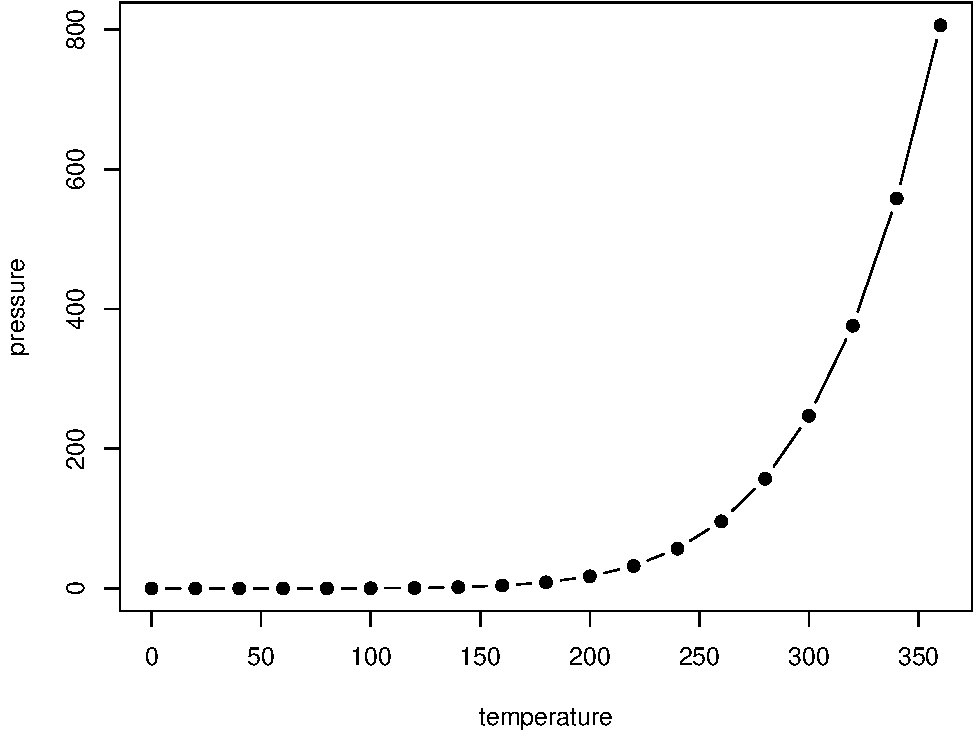
\includegraphics[width=0.8\linewidth]{apuntes_2020_files/figure-latex/nice-fig-1} 

}

\caption{Here is a nice figure!}\label{fig:nice-fig}
\end{figure}

Reference a figure by its code chunk label with the \texttt{fig:} prefix, e.g., see Figure \ref{fig:nice-fig}. Similarly, you can reference tables generated from \texttt{knitr::kable()}, e.g., see Table \ref{tab:nice-tab}.

\begin{Shaded}
\begin{Highlighting}[]
\NormalTok{knitr}\OperatorTok{::}\KeywordTok{kable}\NormalTok{(}
  \KeywordTok{head}\NormalTok{(iris, }\DecValTok{20}\NormalTok{), }\DataTypeTok{caption =} \StringTok{'Here is a nice table!'}\NormalTok{,}
  \DataTypeTok{booktabs =} \OtherTok{TRUE}
\NormalTok{)}
\end{Highlighting}
\end{Shaded}

\begin{table}

\caption{\label{tab:nice-tab}Here is a nice table!}
\centering
\begin{tabular}[t]{rrrrl}
\toprule
Sepal.Length & Sepal.Width & Petal.Length & Petal.Width & Species\\
\midrule
5.1 & 3.5 & 1.4 & 0.2 & setosa\\
4.9 & 3.0 & 1.4 & 0.2 & setosa\\
4.7 & 3.2 & 1.3 & 0.2 & setosa\\
4.6 & 3.1 & 1.5 & 0.2 & setosa\\
5.0 & 3.6 & 1.4 & 0.2 & setosa\\
\addlinespace
5.4 & 3.9 & 1.7 & 0.4 & setosa\\
4.6 & 3.4 & 1.4 & 0.3 & setosa\\
5.0 & 3.4 & 1.5 & 0.2 & setosa\\
4.4 & 2.9 & 1.4 & 0.2 & setosa\\
4.9 & 3.1 & 1.5 & 0.1 & setosa\\
\addlinespace
5.4 & 3.7 & 1.5 & 0.2 & setosa\\
4.8 & 3.4 & 1.6 & 0.2 & setosa\\
4.8 & 3.0 & 1.4 & 0.1 & setosa\\
4.3 & 3.0 & 1.1 & 0.1 & setosa\\
5.8 & 4.0 & 1.2 & 0.2 & setosa\\
\addlinespace
5.7 & 4.4 & 1.5 & 0.4 & setosa\\
5.4 & 3.9 & 1.3 & 0.4 & setosa\\
5.1 & 3.5 & 1.4 & 0.3 & setosa\\
5.7 & 3.8 & 1.7 & 0.3 & setosa\\
5.1 & 3.8 & 1.5 & 0.3 & setosa\\
\bottomrule
\end{tabular}
\end{table}

You can write citations, too. For example, we are using the \textbf{bookdown} package \citep{R-bookdown} in this sample book, which was built on top of R Markdown and \textbf{knitr} \citep{xie2015}.

\hypertarget{introducciuxf3n}{%
\chapter*{Introducción}\label{introducciuxf3n}}
\addcontentsline{toc}{chapter}{Introducción}

Son ya unos cuantos años los que llevo impartiendo docencia de economía y administración de empresas. Desde mis primeras clases, allá por el año 2010, he ido creando y mejorando los distintos materiales que he ido utilizando.

Sin embargo, con el paso del tiempo, he ido notando que más allá de unas buenas transparencias y una buena colección de ejercicios, problemas y prácticas, lo que sin duda puede ser una diferencia es tener unos buenos apuntes que vayan más allá de las meras enumeraciones y definiciones en las que se suelen convertir las transparencias docentes, y marquen un determinado discurso y permitan profundizar un poco en los conceptos explicados.

Lo ideal sin duda alguna era poder recomendar a mis alumnos un libro de referencia con el que poder seguir la asignatura. Afortunadamente manuales de introducción a la economía y a la administración de empresas hay muchos. Sin embargo, recomendar un libro de 400-500 páginas para un curso introductorio en el que ese contenido se puede ver en 5-8 semanas de clase es, desde mi punto de vista, un pequeño despropósito.

Aunque todos pensamientos estaban en mi cabeza, y parecía tener clara la necesidad de tener que fabricarme algo a mi gusto y totalmente adaptado, me faltaba la forma de articularlo. Después de unos años trasnteando con \texttt{R}, lenguaje de programación que poco a poco he ido aprendiendo y con el que he ido descubriendo como hacer cada día más cosas, llegué hasta el paquete \href{https://bookdown.org/}{Bookdown}. Más o menos, y de una forma muy breve, es un paquete que permite crear una estructura de libro utilizando el lenguaje \emph{Markdown}. ¿Ventajas que le veo? Tener actualizado y online (y por tanto disponible para mis alumnos) este compendio de apuntes.

Espero poder decir dentro de un par de años que este experimento ha fraguado correctamente, y que quienes lo estáis leyendo, podéis tener aquí algo así como un que os sirva para el estudio y nos permita dedicar el tiempo de clase a interiorizar los conceptos más que a aprender sobre ellos.

Sea como fuera, aquí está este documento.

\hypertarget{por-quuxe9-leer-este-libro}{%
\section*{¿Por qué leer este libro?}\label{por-quuxe9-leer-este-libro}}
\addcontentsline{toc}{section}{¿Por qué leer este libro?}

Se me ocurre una razón fundamental: soy tu profesor y te lo he recomendado. Si es así, bueno, supongo que lo mejor que puedes hacer es hacerme caso y usar este documento como base para tu estudio y seguir la asignatura.

Puede sin embargo que por otra razón del destino hayas acabado aquí. En ese caso, supongo que habrá algún aspecto del libro que pueda serte de ayuda. Sinceramente, espero que así sea.

\hypertarget{estructura-del-libro}{%
\section*{Estructura del libro}\label{estructura-del-libro}}
\addcontentsline{toc}{section}{Estructura del libro}

El documento está dividido en dos grandes bloques. Un primer apartado de carácter más básico e introductorio enfocado principalmente a una asignatura general de general y administración de empresas de nivel de grado. Luego hay un segundo apartado más aplicado, con conocimiento más avanzado, pensado para una asignatura de nivel de máster.

Sin embargo, puede suceder (y de hecho sucede) que existan apartados o temas mezclados, en los que se empiece dando un concepto y definición y se continúe avanzando hasta un nivel aplicado. Si se ha optado por este enfoque en algunos temas es por mantener el hilo de desarrollo y no hacer ``dar vueltas'' al lector.

\hypertarget{agradecimientos}{%
\section*{Agradecimientos}\label{agradecimientos}}
\addcontentsline{toc}{section}{Agradecimientos}

Es de rigor aquí también agradecer a los alumnos que han formado parte de este proceso, porque gracias a los comentarios e interés de algunos de ellos, algunos apartados han ganado en contenidos, calidad y ejemplos.

Voy a permitir el destacar algunos de ellos, que sin duda han colaborado y ayudado más a la elaboración del documento:

\begin{itemize}
\tightlist
\item
  David Fernández Díaz (Curso 2018/2019, Grado en Ingeniería de los Recursos Energéticos)
\end{itemize}

\hypertarget{literature}{%
\chapter{Literature}\label{literature}}

Here is a review of existing methods.

\hypertarget{methods}{%
\chapter{Methods}\label{methods}}

We describe our methods in this chapter.

\hypertarget{applications}{%
\chapter{Applications}\label{applications}}

Some \emph{significant} applications are demonstrated in this chapter.

\hypertarget{example-one}{%
\section{Example one}\label{example-one}}

\hypertarget{example-two}{%
\section{Example two}\label{example-two}}

\hypertarget{final-words}{%
\chapter{Final Words}\label{final-words}}

We have finished a nice book.

\hypertarget{part-economuxeda-y-administraciuxf3n-de-empresas}{%
\part{Economía y Administración de Empresas}\label{part-economuxeda-y-administraciuxf3n-de-empresas}}

\hypertarget{quuxe9-es-la-economuxeda}{%
\chapter{¿Qué es la economía?}\label{quuxe9-es-la-economuxeda}}

Según Mick Jagger (el que por cierto posee un título en economía de la London School of Economics) y los Rolling Stones, \href{https://www.youtube.com/watch?v=oqMl5CRoFdk}{``You Can't Always Get What You Want''}, o lo que es lo mismo, ``no puedes siempre conseguir lo que quieres''.

¿Por qué no podemos conseguirlo? Porque todos nosotros (los que a partir de ahora nos llamaremos sujetos económicos y que posteriormente definiremos en profundidad) tenemos por lo general necesidades ilimitadas. Si queremos satisfacer estas necesidades, requeriremos de recursos, que al contrario de lo que sucede con nuestras necesidades, no son ilimitados sino generalmente escasos.

La economía se puede definir como la ciencia que dedica sus esfuerzos al estudio de la forma en que los individuos eligen en condiciones de escasez y de las consecuencias de esas elecciones para la sociedad. En la antigua Grecia, economía hacía referencia a ``administrar el patrimonio'', por eso se define como ``la ciencia de la elección'': administrar es elegir entre distintas opciones (Jose Sande, 2015).

La economía es la ciencia que estudia el modo en el que una sociedad gestiona sus recursos (Mankiw, 2002). Uno de los objetivos de la economía es buscar cómo deben asignarse los recursos disponibles para obtener la máxima utilidad de los mismos (o dicho de otra manera, el máximo beneficio). Para ello, a veces la economía recurre a modelos que ayudan a comprender y predecir la realidad. Algunos de ellos son el flujo circular de la renta o la curva frontera de posibilidades de producción.

La \textbf{microeconomia} es una rama de la economía la cual estudia el comportamiento de los agentes individuales (hogares, empresas, sector público) y el funcionamiento de los mercados para asignar los recursos escasos a los distintos usos alternativos.
También estudia como se forman los precios mediante la interacción de los hogares y de las empresas en los distintos mercados.

La \textbf{macroeconomia} es otra rama de la economía que se encarga del estudio de los fenómenos que afectan al conjunto de los grandes agregados económicos (Renta Nacional, PIB\ldots), que nos permiten obtener una visión global de la economía de un país.
Su objetivo principal es comprender y mejorar los resultados de la economía en su entorno mas global.

\hypertarget{los-agentes-econuxf3micos}{%
\section{Los agentes económicos}\label{los-agentes-econuxf3micos}}

Los protagonistas de las actividades económicas somos todos los ciudadanos, también llamados agentes económicos en el entorno de la vida económica. Dependiendo del papel que se juega en la actividad dentro de nuestro sistema, se agrupa en una de estas tres categorías:

\begin{itemize}
\tightlist
\item
  Economía doméstica: Su función es el consumo y el objetivo la máxima satisfacción con unas limitaciones de renta y preferencias.
\item
  Empresas: Se basan en la producción y en el máximo beneficio con limitaciones de presupuesto financiero y tecnología.
\item
  Sector público: Su función es la regulación suministro de bienes públicos y el objetivo es el máximo bienestar económico y colectivo con las limitaciones de los ingresos públicos.
\end{itemize}

\hypertarget{la-escasez-y-el-problema-de-tener-que-decidir}{%
\section{La escasez y el problema de tener que decidir}\label{la-escasez-y-el-problema-de-tener-que-decidir}}

Como hemos dicho anteriormente, los sujetos económicos nos enfrentamos en nuestro día a día a la escasez. La escasez no entendida como un problema tecnológico, sino de disparidad
entre nuestros deseos y los medios de los que disponemos para satisfacerlos.
Por lo tanto, igualmente nos encontramos día a día frente a decisiones que se nos plantean para decidir qué necesidades satisfacemos primero y a cuales debemos renunciar. A la hora de tomar estas decisiones, los sujetos económicos nos basamos en varios principios básicos, presentes en todas y cada una de nuestras decisiones.

\begin{itemize}
\tightlist
\item
  Principio de escasez
\item
  Principio Coste-Beneficio
\item
  Principio de los incentivos
\item
  Principio de eficiencia y equidad
\end{itemize}

\hypertarget{los-costes-econuxf3micos-en-la-toma-de-decisiones}{%
\section{Los costes económicos en la toma de decisiones}\label{los-costes-econuxf3micos-en-la-toma-de-decisiones}}

La economía nos enseña que ``no hay nada gratis''. Dicho de otra forma, todas nuestras decisiones tienen un coste asociado, que es lo que denominamos coste de oportunidad.

\begin{quote}
\textbf{Coste de oportunidad}: es el coste asociado a aquello a lo que se renuncia cuando se toma una decisión. Más concretamente, el coste de oportunidad de un bien o servicio es la cantidad de otros bienes o servicios a la que se debe renunciar para obtenerlo.
\end{quote}

Pongamos un ejemplo. Supongamos que es media mañana y es la hora de nuestra pausa para el almuerzo. Después de haber desayunado a primera hora del día, a esa hora puede ser bastante normal que tengamos tanto hambre como algo de sed. Sin embargo, hemos salido apresurados de casa por la mañana y hemos dejado olvidado nuestro monedero. Tan sólo tenemos 1€.
En el bar nos ofrecen bebida y comida, pero el refresco que deseamos cuesta 1€ y el pincho de tortilla que nos gusta tiene un precio de 1€ también. Debemos elegir, y debemos renunciar. Si elegimos saciar nuestra sed, y pedimos el refresco, estamos sacrificando el pincho de tortilla. Mantenernos con hambre es por tanto nuestro coste de oportunidad de elegir el refresco. El coste de oportunidad de elegir comer un pincho de tortilla es mantenernos con sed.

Además de este concepto de coste de oportunidad, en nuestras tomas de decisiones aparecen otros costes que también nos influyen desde el punto de vista económico.

\begin{quote}
\textbf{Coste irrecuperable}: es un coste que en cualquiera de las opciones de decisión que nos planteemos, está presente. Al ser un coste que vamos a tener que asumir siempre, independientemente de nuestra decisión, no debería influir en la toma de decisión.
\end{quote}

Sigamos con nuestro ejemplo y supongamos ahora que además de lo anterior, para llegar al bar debemos cruzar una gran avenida, y tenemos la mala suerte de que en este momento está lloviendo a mares. Volviendo a la situación anterior, tanto si elegimos comernos el pincho de tortilla como bebernos el refresco, tendremos un coste adicional, que es estar mojados por la lluvia. Este es un coste irrecuperable.

\begin{quote}
\textbf{Coste de transacción}: es un coste en el que necesariamente incurrimos al realizar un intercambio económico, o más precisamente, una transacción en un mercado.
\end{quote}

La existencia de estos costes de transacción fue desarrollada por primera vez por el economista Ronald Coase en su artículo The Nature of the Firm (1937). Coase explica que ``cuando se desea operar una transacción en un mercado, es necesario investigar a los contratistas, proporcionarles ciertas informaciones necesarias y establecer las condiciones del contrato, llevar a cabo las negociaciones que instauren un verdadero mercado, establecer una estructura de control de las respectivas prestaciones de obligaciones de las partes, etc.'' \citep{coase1937}. Sin embargo, es a John Kenneth Arrow a quien se debe el uso del término ``coste de transacción'' \citep{arrow1969}.

Los costes de transacción los podemos agrupar en tres grandes categorías:

\begin{itemize}
\tightlist
\item
  Costes de investigación e información, que son los costes en los que incurrimos cuando queremos saber si el producto que queremos intercambiar está disponible en el mercado, quién tiene el menor precio, etc. Incluyen la recopilación de la información, la comparación de las alternativas, el análisis de su relación calidad/precio, etc.
\item
  Costes de negociación y de decisión, que son los costes necesarios para llegar a un acuerdo con la otra parte de la negociación (tiempo, redacción de documentos).
\item
  Costes de vigilancia y de ejecución, que son los costes necesarios para asegurar que ambas parten cumplen con lo pactado según los términos acordados, así como los costes de tomar acciones si no se cumple con lo previsto.
\end{itemize}

Imagina que has ido de viaje a la vecina Portugal (Oporto por poner un lugar algo más concreto) por vacaciones y deseas traer un buen regalo a la familia: un juego de toallas. Recorrerte durante toda una tarde la zona más turística de Oporto buscando las mejores ofertas, así como los diseños más adecuados y las toallas de mejor calidad supone un coste de investigación e información. Una vez que has decidido el local con el mejor género y mejores precios, llegar a un acuerdo con el propietario por el juego de 6 toallas que quieres adquirir, supone un coste de negociación. El arte del regateo. Por último, comprobar que el género adquirido es de algodón puro y de buena calidad (con envío de muestra a un laboratorio independiente para su análisis si nos ponemos exquisitos) sería un coste de vigilancia y ejecución. Todos ellos, serían ejemplos de costes de transacción.

\hypertarget{oferta-y-demanda}{%
\chapter{Oferta y demanda}\label{oferta-y-demanda}}

La oferta y la demanda son dos conceptos recurrentes que aparecen cuando hablamos de economía. Son las dos fuerzas o palancas que hacen que las economías de mercado funcionen. La oferta y la demanda determinan la cantidad que se produce de cada bien y el precio al que debe venderse. Y esto lo hacen al interactuar en los mercados. El mercado de un producto está formado por todos los vendedores y compradores de un producto, y por lo tanto, por su oferta y su demanda.

\hypertarget{la-demanda}{%
\section{La demanda}\label{la-demanda}}

La demanda es la cantidad que los consumidores (compradores) desean y pueden comprar en funcion del precio.

\begin{quote}
\textbf{LEY DE LA DEMANDA}:
Manteniéndose todo lo demas constante (\emph{ceteris paribus}), cuando aumenta el precio de un bien, la demanda baja.
\end{quote}

La demanda de mercado de un determinado bien es la suma de todas las demandas individuales que lo integran.

La razón por la que cuando el precio del bien aumenta la cantidad demandada por todos los consumidores disminuye es doble. Por un lado, cuando aumenta el precio de un bien algunos consumidores que previamente lo adquirían dejarán de hacerlo o lo comprarán en menor cuantía y buscarán otros bienes que lo sustituirán. Esto se conoce como efecto sustitución, en el sentido de que el bien o servicio que se encarece relativamente tiende a ser sustituido por otros que ahora resultan más baratos.

Por otro lado, los consumidores cuando un bien se encarece demandarán menos unidades del mismo porque la elevación del precio ha reducido la capacidad adquisitiva de la renta, y esto hará que se pueda comprar menos de todos los bienes y, en particular, del que estamos considerando. Este hecho se conoce como el efecto renta, e indica que un incremento en los precios de un bien, disminuye la capacidad adquisitiva de los consumidores para un nivel de renta dado. Ante esta circunstancia los consumidores se verán motivados a reducir la compra de todos los bienes o servicios.

\hypertarget{la-curva-de-demanda}{%
\subsection{La curva de demanda}\label{la-curva-de-demanda}}

La curva de demanda es la representación gráfica de la relación entre el precio de un bien y la cantidad demandada. Al trazar la curva de demanda suponemos que se mantienen constantes los demás factores, excepto el precio, que puedan afectar a la cantidad demandada.

La función de demanda es una relación matemática que recoge la relación entre la cantidad demandada de un bien, su precio y otras variables.

\hypertarget{movimientos-de-la-curva-de-demanda}{%
\subsection{Movimientos de la curva de demanda}\label{movimientos-de-la-curva-de-demanda}}

Cuando varía el precio de un bien, el desplazamiento se produce a lo largo de la curva de demanda Sin embargo, la curva de oferta se desplaza cuando se altera cualquiera de los factores que inciden en la demanda distinto del precio:

\begin{itemize}
\tightlist
\item
  La renta o ingreso de los consumidores (léase \emph{bienes normales} o \emph{bienes inferiores}).
\item
  Los precios de los bienes relacionados (léase \emph{bienes complementarios}, \emph{bienes sustitutivos} o \emph{bienes independientes}).
\item
  Los gustos o preferencias de los consumidores.
\item
  El tamaño del mercado o el número de consumidores.
\end{itemize}

\hypertarget{la-oferta}{%
\section{La oferta}\label{la-oferta}}

La oferta es la cantidad que los productores (vendedores) quieren y pueden vender a los distintos precios.

\begin{quote}
\textbf{LEY DE LA OFERTA}:
Manteniéndose todo lo demas constante (\emph{ceteris paribus}), cuando aumenta el precio de un bien, la oferta aumenta.
\end{quote}

La oferta de mercado de un determinado bien es la suma de todas las oferta individuales que lo integran.

\hypertarget{la-curva-de-oferta}{%
\subsection{La curva de oferta}\label{la-curva-de-oferta}}

La curva de demanda es la representación gráfica de la relación entre el precio de un bien y la cantidad ofrecida Al trazar la curva de oferta suponemos que se mantienen constantes las demás variables, excepto el precio, que puedan afectar a la cantidad ofertada.

La función de oferta es una relación matemática que recoge la relación entre la cantidad demandada de un bien, su precio y las demás variables que influyen en las decisiones de producción.

\hypertarget{movimientos-de-la-curva-de-oferta}{%
\subsection{Movimientos de la curva de oferta}\label{movimientos-de-la-curva-de-oferta}}

Cuando varía el precio de un bien, el desplazamiento se produce a lo largo de la curva de oferta. Sin embargo, la curva de oferta se desplaza cuando se altera cualquiera de los factores que inciden en la oferta distinto del precio:

\begin{itemize}
\tightlist
\item
  El precio de los factores productivos.
\item
  La tecnología existente.
\item
  El número de empresas existentes en el mercado.
\end{itemize}

\hypertarget{el-punto-de-equilibrio}{%
\section{El punto de equilibrio}\label{el-punto-de-equilibrio}}

Cuando consumidores y productores se ponen en contacto para intercambiar un bien, cada uno de ellos con sus respectivas curvas de demanda y oferta, existe un punto en el que ambos agentes se ponen de acuerdo. Existen multitud de precios en los que los planes de cada uno de ellos no coinciden, pero existe un único punto en el que se da la coincidencia. Este es el punto de equilibrio del mercado y nos proporciona información sobre la cantidad (demandada y ofertada) y el precio de equilibrio.

\begin{quote}
\textbf{Punto de equilibrio}:
Es el punto en el que coinciden oferta y demanda. El precio de equilibrio es aquel en el cual la cantidad demandada es igual a la cantidad ofertada, siendo ésta la cantidad de equilibrio.
\end{quote}

En el punto de equilibrio, dado que los deseos de los consumidores y de los productores coinciden, no hay escasez ni excedente del bien.
Un exceso de oferta o excedente, es la situación en la que la cantidad ofrecida es mayor que la demandada.
Un exceso de demanda o escasez, es la situación en la que la cantidad demandada es mayor que la ofrecida.

Si a partir de una posición de equilibrio tienen lugar desplazamientos simultáneos de las curvas de demanda y de oferta, el impacto sobre el precio y la cantidad de equilibrio será ambiguo pues dependerá de la magnitud del cambio experimentado por cada una de las curvas.

\hypertarget{la-elasticidad}{%
\chapter{La elasticidad}\label{la-elasticidad}}

Para explicar el comportamiento de los consumidores podemos aceptar como punto de partida que los individuos tienden a elegir aquellos bienes y servicios que valoran más, es decir, aquellos que les reportan una mayor utilidad o satisfacción. En otras palabras, vamos a suponer que los individuos maximizan su utilidad, lo que implica que eligen el conjunto de bienes de consumo que más prefieren.

La utilidad es el sentimiento subjetivo de placer o satisfacción que una persona experimenta como consecuencia de consumir un bien o un servicio.

El principio equimarginal o de la igualdad de las utilidades marginales por euro gastado establece que cada bien se demanda hasta el punto en que la utilidad marginal del último euro gastado en él es exactamente igual a la utilidad marginal del último euro gastado en cualquier otro bien.

El excedente del consumidor de un bien es la diferencia entre la cantidad máxima que éste estaría dispuesto a pagar por el número de unidades del bien que demanda y la cantidad que realmente paga en el mercado. El excedente del consumidor es la diferencia entre la utilidad total de un bien y su valor total de mercado.

\hypertarget{elasticidad}{%
\section{Elasticidad}\label{elasticidad}}

La elasticidad es un concepto económico introducido por el economista inglés Alfred Marshall, para cuantificar la variación experimentada por una variable al cambiar otra. El concepto económico de la elasticidad parte de la existencia de dos variables, entre las que existe una cierta dependencia, por ejemplo el número de automóviles vendidos y el precio de los automóviles. La elasticidad mide la sensibilidad de la cantidad de automóviles vendidos ante la variación del precio de los mismos.

\hypertarget{elasticidad-de-la-demanda}{%
\section{Elasticidad de la demanda}\label{elasticidad-de-la-demanda}}

La elasticidad es una medida de la sensibilidad de la cantidad demandada o de la cantidad ofrecida ante el cambio en alguno de sus factores determinantes.

La demanda es elástica si la elasticidad precio de la demanda es mayor que 1; es inelástica si es menor que 1, y es de elasticidad unitaria si es igual a 1.

\hypertarget{elasticidad-de-la-oferta}{%
\section{Elasticidad de la oferta}\label{elasticidad-de-la-oferta}}

El concepto de elasticidad que se ha aplicado a la curva de demanda también puede referirse a la curva de la oferta.

La elasticidad es un indicador que nos sirve para medir los cambios de una variable cuando cambia otra. Hay dos tipos de elasticidad, segun: A)Precio de la demanda: Mide que es lo que sucede a la demanda cuando cambia el precio. B) Precio de la oferta: Mide los cambios en la oferta cuando varia el precio. Ambas varioaciones cuando son mayores que el 1\% se llaman elasticas, y cuando estan entre el 0 y 1\%, inelasticas.

\hypertarget{mercados}{%
\chapter{Mercados}\label{mercados}}

Un mercado es toda institución social en la que los bienes y servicios, así como los factores productivos, se intercambian. Permite una definición dual: desde un punto de vista puramente físico haciéndose referencia al lugar donde se producen los intercambios; desde un punto de vista más formal o institucional, hace referencia a la conjunción de compradores y vendedores.

Un mercado está compuesto por dos elementos fundamentales: por un lado la oferta, definida por la actitud de los productores; y por otro lado la demanda, determinada por el comportamiento de los consumidores.

Las principales caracteristicas que definen la estructura de un mercado son las siguientes:

\begin{enumerate}
\def\labelenumi{\arabic{enumi}.}
\tightlist
\item
  Numero de agentes.
\item
  Grado de competencia entre los vendedores.
\item
  Tipo de producto. Homogeneo o heterogeneo.
\item
  La existencia o no de barreras de entrada. Las cuales son el impedimento que hace que alguien no pueda entrar en un mercado. Dentro de estas distinguimos ciertos tipos:

  \begin{itemize}
  \tightlist
  \item
    Proceso productivo.
  \item
    Recursos monopolisticos.
  \item
    Patentes legales.
  \end{itemize}
\item
  Control sobre el precio.
\item
  La transparencia. Control sobre la información.
\end{enumerate}

En función de qué situaciones se den para cada una de las características anteriores, se distinguirá una tipología u otra de mercado. En general, se distinguen las siguientes tipologías básicas de mercados: competencia perfecta, monopolio, oligopolio y competencia monopolística.

\hypertarget{competencia-perfecta}{%
\section{Competencia perfecta}\label{competencia-perfecta}}

Los mercados de competencia perfecta se caracterizan porque presentan las siguientes características:

\begin{enumerate}
\def\labelenumi{\arabic{enumi}.}
\tightlist
\item
  Existencia de un número elevado de compradores y vendedores.
\item
  Existe una alta competencia entre los vendedores.
\item
  Los bienes ofrecidos por los distintos vendedores son prácticamente idénticos.
\item
  Las empresas pueden entrar o salir libremente del mercado.
\item
  Las empresas individualmente no tienen capacidad para fijar el precio del producto.
\item
  Existe información perfecta.
\end{enumerate}

\hypertarget{monopolio}{%
\section{Monopolio}\label{monopolio}}

Del griego antiguo mόνος (\emph{mono}, ``uno''), y de πόλλειν, (\emph{polein}, ``vender'').
El caso extremo de un mercado imperfectamente competitivo es el monopolio, ya que sólo hay un único ofertante en la industria. Una empresa es un monopolio si es la única que oferta un producto y si éste no tiene sustitutivos cercanos.

\begin{enumerate}
\def\labelenumi{\arabic{enumi}.}
\tightlist
\item
  Sólo existe un único vendedor.
\item
  No existe compentencia alguna al existir un único vendedor.
\item
  Se comercializa un único producto sin sustitutivos cercanos.
\item
  Generalmente aparecen importantes barreras de entrada al mercado.
\item
  El único vendedor tiene un gran poder a la hora de fijar el precio.
\item
  No existe una gran información sobre los costes del vendedor.
\end{enumerate}

Su objetivo principal es maximizar el beneficio. Encontramos que el precio del producto es mayor que el ingreso marginal
Ejemplos de monopolio son: el agua y las empresas de ferrocaril y autobuses.
Para este tipo de mercados hay diferentes soluciones como: aumentar la competencia y prohibir los monopolios.

\hypertarget{barreras-de-entrada}{%
\subsection{Barreras de entrada}\label{barreras-de-entrada}}

Las barreras a la entrada son factores que limitan la entrada de nuevas empresas en una industria, de forma que, cuando son altas, la industria tendrá pocas empresas y escasas presiones para competir.

\begin{enumerate}
\def\labelenumi{\arabic{enumi}.}
\tightlist
\item
  Las restricciones legales (patentes, las restricciones o concesiones administrativas, existencia de tarifas y cuotas al comercio internacional).
\item
  La publicidad y la diferenciación del producto.
\item
  Costes de entrada elevados.
\end{enumerate}

\hypertarget{oligopolio}{%
\section{Oligopolio}\label{oligopolio}}

Del griego antiguo ὀλιγς (\emph{oligos}, ``poco'', ``pocos''), y de πόλλειν, (\emph{polein}, ``vender'').

Este tipo de mercados esta caracterizado por tener pocos vendedores y muchos compradores, en el cual encontramos una gran competencia entre los vendedores e incluso encontramos pactos. Aqui las decisiones de un sujeto afectan a los demas, lo cual se llama: Interdependencia estrategica.
En estos mercados los vendedores deben elegir entre conseguir el maximo beneficio o cooperar con los demas vendedores. Al coopear encontramos dos tipos de pacto, el cartel, que es un grupo de empresas que trabajan como una sola, y la colusion, en la cual las empresas se reparten el mercado.
Un ejemplo de este mercado son los medicamentos.

\hypertarget{competencia-monopoluxedstica}{%
\section{Competencia monopolística}\label{competencia-monopoluxedstica}}

Las principales caracteristicas de este mercado es que la competencia entre los vendedores es alta dado que hay muchos, al igual que compradores que tambien hay muchos y las empresas tienen que competir por ellos. Podemos encontrar productos diferenciados y algun tipo de barrera al entrar a este mercado, como por ejemplo de tipo legal. Los vendedores tienen algo de control sobre el precio de sus productos y la transparencia es imperfecta.
Observamos algún ejemplo claro como los teléfonos móvil y los pañuelos de papel.

\hypertarget{otras-tipologuxedas}{%
\section{Otras tipologías}\label{otras-tipologuxedas}}

Así como en los monopolios y oligopolios hablábamos de la raíz griega πόλλειν, (\emph{polein}, ``vender''), podemos igualmente encontrarnos con monopsonios y oligopsonios. En este caso, aparece la raíz ψωνιος (\emph{psonios}, ``compra''), por lo que nos van a aparecer mercados en los que el poder lo tienen los compradores, bien porque sólamente hay uno (monopsonios) o porque hay muy pocos (oligopsonios).

Ejemplo de este tipo de mercados suele ser el sistema nacional de salud y su compra centralizada de medicamentos: un único comprador que engloba la compra de todos los medicamentos para el país, otorgando por tanto un poder importante a la hora de negociar el precio de compra. Cuando este sistema se transfiere a las comunidades autónomas, surgen distintos sistemas de salud encargados de realizar esta compra, por lo que se transforma el mercado en un oligopsonio. Los sistemas pierden algo de poder, pero al seguir siendo un número reducido, pueden seguir influyendo sobre el precio, y por supuesto, pueden agruparse para aumentar su poder al igual que sucedía en los oligopolios.

\hypertarget{los-fallos-de-mercado}{%
\chapter{Los fallos de mercado}\label{los-fallos-de-mercado}}

el funcionamiento de los mercados en ocasiones falla. Estos fallos de mercado se pueden sintetizar en la siguiente tipología:
A) Competencia imperfecta.
B) Externalidades.
C) Información imperfecta.

\begin{quote}
Un fallo del mercado tiene lugar cuando un mercado no asigna eficientemente los recursos por sí solo.
\end{quote}

\hypertarget{las-externalidades}{%
\section{Las externalidades}\label{las-externalidades}}

Aparecen externalidades, como la contaminación, que el mercado no aborda. Así, una industria que produce papel puede contaminar las aguas de un río al que vierte sus residuos. La actividad de la industria perjudica a los agricultores que utilizan el agua del río y los precios de producir papel no reflejan el perjuicio que se está ocasionando a los agricultores (véase Capítulo 8).

\hypertarget{competencia-imperfecta}{%
\section{Competencia imperfecta}\label{competencia-imperfecta}}

Existen mercados en los que la competencia es imperfecta. Como veremos en el Capítulo 6, en muchos mercados uno o más participantes pueden influir sobre los precios, fijando el nivel que les resulte más conveniente.

\hypertarget{informaciuxf3n-imperfecta}{%
\section{Información imperfecta}\label{informaciuxf3n-imperfecta}}

La información en muchos casos es imperfecta. En algunos mercados el supuesto de información plena está lejos de la realidad, lo que supone un fallo del mercado (véase Capítulo 8).

Este tipo de problemas sugiere la conveniencia de que en determinadas circunstancias el Estado pueda intervenir en la economía para tratar de mejorar su funcionamiento tanto a nivel de mercados concretos (esto es, vía políticas microeconómicas) como desde una perspectiva global, esto es, mediante el recurso a las políticas macroeconómicas. Por ello, en los países occidentales es frecuente hablar de economías mixtas.

\hypertarget{mercados-agregados}{%
\chapter{Mercados agregados}\label{mercados-agregados}}

We have finished a nice book.

  \bibliography{book.bib,packages.bib}

\end{document}
